% Created by tikzDevice version 0.12.6 on 2026-08-10 06:16:14
% !TEX encoding = UTF-8 Unicode
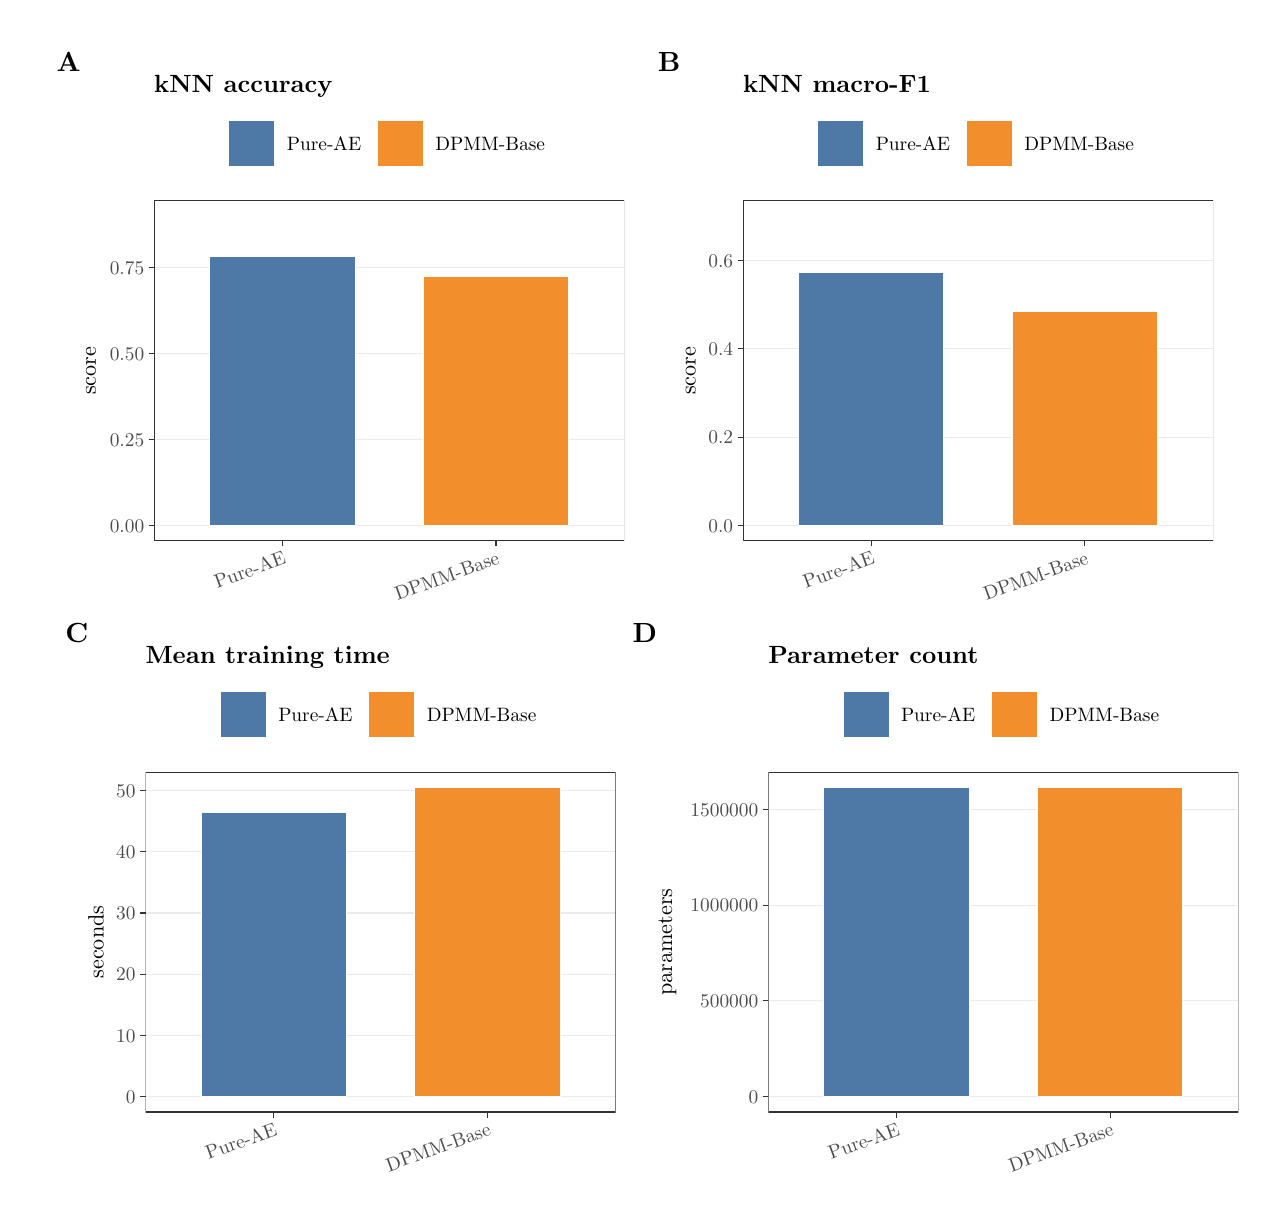
\begin{tikzpicture}[x=1pt,y=1pt]
\definecolor{fillColor}{RGB}{255,255,255}
\path[use as bounding box,fill=fillColor,fill opacity=0.00] (0,0) rectangle (441.01,423.78);
\begin{scope}
\path[clip] (  0.00,  0.00) rectangle (441.01,423.78);
\definecolor{drawColor}{RGB}{255,255,255}
\definecolor{fillColor}{RGB}{255,255,255}

\path[draw=drawColor,line width= 0.6pt,line join=round,line cap=round,fill=fillColor] (  0.00,  0.00) rectangle (441.01,423.78);
\end{scope}
\begin{scope}
\path[clip] (  5.50,211.89) rectangle (220.50,418.28);
\definecolor{drawColor}{RGB}{255,255,255}
\definecolor{fillColor}{RGB}{255,255,255}

\path[draw=drawColor,line width= 0.6pt,line join=round,line cap=round,fill=fillColor] (  5.50,211.89) rectangle (220.50,418.28);
\end{scope}
\begin{scope}
\path[clip] (220.50,211.89) rectangle (435.51,418.28);
\definecolor{drawColor}{RGB}{255,255,255}
\definecolor{fillColor}{RGB}{255,255,255}

\path[draw=drawColor,line width= 0.6pt,line join=round,line cap=round,fill=fillColor] (220.50,211.89) rectangle (435.51,418.28);
\end{scope}
\begin{scope}
\path[clip] (  8.46,212.32) rectangle (217.54,417.85);
\definecolor{drawColor}{RGB}{255,255,255}
\definecolor{fillColor}{RGB}{255,255,255}

\path[draw=drawColor,line width= 0.4pt,line join=round,line cap=round,fill=fillColor] (  8.46,212.32) rectangle (217.54,417.85);
\end{scope}
\begin{scope}
\path[clip] ( 45.71,238.34) rectangle (215.54,361.19);
\definecolor{fillColor}{RGB}{255,255,255}

\path[fill=fillColor] ( 45.71,238.34) rectangle (215.54,361.19);
\definecolor{drawColor}{gray}{0.92}

\path[draw=drawColor,line width= 0.4pt,line join=round] ( 45.71,243.92) --
	(215.54,243.92);

\path[draw=drawColor,line width= 0.4pt,line join=round] ( 45.71,274.94) --
	(215.54,274.94);

\path[draw=drawColor,line width= 0.4pt,line join=round] ( 45.71,305.97) --
	(215.54,305.97);

\path[draw=drawColor,line width= 0.4pt,line join=round] ( 45.71,336.99) --
	(215.54,336.99);
\definecolor{drawColor}{RGB}{255,255,255}
\definecolor{fillColor}{RGB}{78,121,167}

\path[draw=drawColor,line width= 0.3pt,fill=fillColor] ( 65.78,243.92) rectangle (118.27,341.21);
\definecolor{fillColor}{RGB}{242,142,43}

\path[draw=drawColor,line width= 0.3pt,fill=fillColor] (142.97,243.92) rectangle (195.47,333.89);
\definecolor{drawColor}{gray}{0.20}

\path[draw=drawColor,line width= 0.4pt,line join=round,line cap=round] ( 45.71,238.34) rectangle (215.54,361.19);
\end{scope}
\begin{scope}
\path[clip] (  0.00,  0.00) rectangle (441.01,423.78);
\definecolor{drawColor}{gray}{0.30}

\node[text=drawColor,anchor=base east,inner sep=0pt, outer sep=0pt, scale=  0.70] at ( 42.11,241.51) {0.00};

\node[text=drawColor,anchor=base east,inner sep=0pt, outer sep=0pt, scale=  0.70] at ( 42.11,272.53) {0.25};

\node[text=drawColor,anchor=base east,inner sep=0pt, outer sep=0pt, scale=  0.70] at ( 42.11,303.56) {0.50};

\node[text=drawColor,anchor=base east,inner sep=0pt, outer sep=0pt, scale=  0.70] at ( 42.11,334.58) {0.75};
\end{scope}
\begin{scope}
\path[clip] (  0.00,  0.00) rectangle (441.01,423.78);
\definecolor{drawColor}{gray}{0.20}

\path[draw=drawColor,line width= 0.4pt,line join=round] ( 43.71,243.92) --
	( 45.71,243.92);

\path[draw=drawColor,line width= 0.4pt,line join=round] ( 43.71,274.94) --
	( 45.71,274.94);

\path[draw=drawColor,line width= 0.4pt,line join=round] ( 43.71,305.97) --
	( 45.71,305.97);

\path[draw=drawColor,line width= 0.4pt,line join=round] ( 43.71,336.99) --
	( 45.71,336.99);
\end{scope}
\begin{scope}
\path[clip] (  0.00,  0.00) rectangle (441.01,423.78);
\definecolor{drawColor}{gray}{0.20}

\path[draw=drawColor,line width= 0.4pt,line join=round] ( 92.02,236.34) --
	( 92.02,238.34);

\path[draw=drawColor,line width= 0.4pt,line join=round] (169.22,236.34) --
	(169.22,238.34);
\end{scope}
\begin{scope}
\path[clip] (  0.00,  0.00) rectangle (441.01,423.78);
\definecolor{drawColor}{gray}{0.30}

\node[text=drawColor,rotate= 20.00,anchor=base east,inner sep=0pt, outer sep=0pt, scale=  0.70] at ( 93.67,230.20) {Pure-AE};

\node[text=drawColor,rotate= 20.00,anchor=base east,inner sep=0pt, outer sep=0pt, scale=  0.70] at (170.87,230.20) {DPMM-Base};
\end{scope}
\begin{scope}
\path[clip] (  0.00,  0.00) rectangle (441.01,423.78);
\definecolor{drawColor}{RGB}{0,0,0}

\node[text=drawColor,rotate= 90.00,anchor=base,inner sep=0pt, outer sep=0pt, scale=  0.80] at ( 24.67,299.76) {score};
\end{scope}
\begin{scope}
\path[clip] (  0.00,  0.00) rectangle (441.01,423.78);
\definecolor{fillColor}{RGB}{255,255,255}

\path[fill=fillColor] ( 68.33,369.19) rectangle (192.92,394.54);
\end{scope}
\begin{scope}
\path[clip] (  0.00,  0.00) rectangle (441.01,423.78);
\definecolor{fillColor}{RGB}{255,255,255}

\path[fill=fillColor] ( 72.33,373.19) rectangle ( 89.67,390.54);
\definecolor{drawColor}{RGB}{255,255,255}
\definecolor{fillColor}{RGB}{78,121,167}

\path[draw=drawColor,line width= 0.3pt,fill=fillColor] ( 72.69,373.55) rectangle ( 89.32,390.18);
\end{scope}
\begin{scope}
\path[clip] (  0.00,  0.00) rectangle (441.01,423.78);
\definecolor{fillColor}{RGB}{255,255,255}

\path[fill=fillColor] (125.99,373.19) rectangle (143.34,390.54);
\definecolor{drawColor}{RGB}{255,255,255}
\definecolor{fillColor}{RGB}{242,142,43}

\path[draw=drawColor,line width= 0.3pt,fill=fillColor] (126.35,373.55) rectangle (142.98,390.18);
\end{scope}
\begin{scope}
\path[clip] (  0.00,  0.00) rectangle (441.01,423.78);
\definecolor{drawColor}{RGB}{0,0,0}

\node[text=drawColor,anchor=base west,inner sep=0pt, outer sep=0pt, scale=  0.70] at ( 93.67,379.46) {Pure-AE};
\end{scope}
\begin{scope}
\path[clip] (  0.00,  0.00) rectangle (441.01,423.78);
\definecolor{drawColor}{RGB}{0,0,0}

\node[text=drawColor,anchor=base west,inner sep=0pt, outer sep=0pt, scale=  0.70] at (147.34,379.46) {DPMM-Base};
\end{scope}
\begin{scope}
\path[clip] (  0.00,  0.00) rectangle (441.01,423.78);
\definecolor{drawColor}{RGB}{0,0,0}

\node[text=drawColor,anchor=base west,inner sep=0pt, outer sep=0pt, scale=  0.90] at ( 45.71,400.53) {\bfseries kNN accuracy};
\end{scope}
\begin{scope}
\path[clip] (  0.00,  0.00) rectangle (441.01,423.78);
\definecolor{drawColor}{RGB}{0,0,0}

\node[text=drawColor,anchor=base,inner sep=0pt, outer sep=0pt, scale=  1.00] at ( 14.81,407.84) {\bfseries A};
\end{scope}
\begin{scope}
\path[clip] (225.68,212.32) rectangle (430.34,417.85);
\definecolor{drawColor}{RGB}{255,255,255}
\definecolor{fillColor}{RGB}{255,255,255}

\path[draw=drawColor,line width= 0.4pt,line join=round,line cap=round,fill=fillColor] (225.68,212.32) rectangle (430.34,417.85);
\end{scope}
\begin{scope}
\path[clip] (258.50,238.34) rectangle (428.34,361.19);
\definecolor{fillColor}{RGB}{255,255,255}

\path[fill=fillColor] (258.50,238.34) rectangle (428.34,361.19);
\definecolor{drawColor}{gray}{0.92}

\path[draw=drawColor,line width= 0.4pt,line join=round] (258.50,243.92) --
	(428.34,243.92);

\path[draw=drawColor,line width= 0.4pt,line join=round] (258.50,275.83) --
	(428.34,275.83);

\path[draw=drawColor,line width= 0.4pt,line join=round] (258.50,307.74) --
	(428.34,307.74);

\path[draw=drawColor,line width= 0.4pt,line join=round] (258.50,339.65) --
	(428.34,339.65);
\definecolor{drawColor}{RGB}{255,255,255}
\definecolor{fillColor}{RGB}{78,121,167}

\path[draw=drawColor,line width= 0.3pt,fill=fillColor] (278.57,243.92) rectangle (331.07,335.19);
\definecolor{fillColor}{RGB}{242,142,43}

\path[draw=drawColor,line width= 0.3pt,fill=fillColor] (355.77,243.92) rectangle (408.26,321.30);
\definecolor{drawColor}{gray}{0.20}

\path[draw=drawColor,line width= 0.4pt,line join=round,line cap=round] (258.50,238.34) rectangle (428.34,361.19);
\end{scope}
\begin{scope}
\path[clip] (  0.00,  0.00) rectangle (441.01,423.78);
\definecolor{drawColor}{gray}{0.30}

\node[text=drawColor,anchor=base east,inner sep=0pt, outer sep=0pt, scale=  0.70] at (254.90,241.51) {0.0};

\node[text=drawColor,anchor=base east,inner sep=0pt, outer sep=0pt, scale=  0.70] at (254.90,273.42) {0.2};

\node[text=drawColor,anchor=base east,inner sep=0pt, outer sep=0pt, scale=  0.70] at (254.90,305.33) {0.4};

\node[text=drawColor,anchor=base east,inner sep=0pt, outer sep=0pt, scale=  0.70] at (254.90,337.24) {0.6};
\end{scope}
\begin{scope}
\path[clip] (  0.00,  0.00) rectangle (441.01,423.78);
\definecolor{drawColor}{gray}{0.20}

\path[draw=drawColor,line width= 0.4pt,line join=round] (256.50,243.92) --
	(258.50,243.92);

\path[draw=drawColor,line width= 0.4pt,line join=round] (256.50,275.83) --
	(258.50,275.83);

\path[draw=drawColor,line width= 0.4pt,line join=round] (256.50,307.74) --
	(258.50,307.74);

\path[draw=drawColor,line width= 0.4pt,line join=round] (256.50,339.65) --
	(258.50,339.65);
\end{scope}
\begin{scope}
\path[clip] (  0.00,  0.00) rectangle (441.01,423.78);
\definecolor{drawColor}{gray}{0.20}

\path[draw=drawColor,line width= 0.4pt,line join=round] (304.82,236.34) --
	(304.82,238.34);

\path[draw=drawColor,line width= 0.4pt,line join=round] (382.02,236.34) --
	(382.02,238.34);
\end{scope}
\begin{scope}
\path[clip] (  0.00,  0.00) rectangle (441.01,423.78);
\definecolor{drawColor}{gray}{0.30}

\node[text=drawColor,rotate= 20.00,anchor=base east,inner sep=0pt, outer sep=0pt, scale=  0.70] at (306.47,230.20) {Pure-AE};

\node[text=drawColor,rotate= 20.00,anchor=base east,inner sep=0pt, outer sep=0pt, scale=  0.70] at (383.67,230.20) {DPMM-Base};
\end{scope}
\begin{scope}
\path[clip] (  0.00,  0.00) rectangle (441.01,423.78);
\definecolor{drawColor}{RGB}{0,0,0}

\node[text=drawColor,rotate= 90.00,anchor=base,inner sep=0pt, outer sep=0pt, scale=  0.80] at (241.37,299.76) {score};
\end{scope}
\begin{scope}
\path[clip] (  0.00,  0.00) rectangle (441.01,423.78);
\definecolor{fillColor}{RGB}{255,255,255}

\path[fill=fillColor] (281.12,369.19) rectangle (405.71,394.54);
\end{scope}
\begin{scope}
\path[clip] (  0.00,  0.00) rectangle (441.01,423.78);
\definecolor{fillColor}{RGB}{255,255,255}

\path[fill=fillColor] (285.12,373.19) rectangle (302.47,390.54);
\definecolor{drawColor}{RGB}{255,255,255}
\definecolor{fillColor}{RGB}{78,121,167}

\path[draw=drawColor,line width= 0.3pt,fill=fillColor] (285.48,373.55) rectangle (302.11,390.18);
\end{scope}
\begin{scope}
\path[clip] (  0.00,  0.00) rectangle (441.01,423.78);
\definecolor{fillColor}{RGB}{255,255,255}

\path[fill=fillColor] (338.79,373.19) rectangle (356.13,390.54);
\definecolor{drawColor}{RGB}{255,255,255}
\definecolor{fillColor}{RGB}{242,142,43}

\path[draw=drawColor,line width= 0.3pt,fill=fillColor] (339.14,373.55) rectangle (355.77,390.18);
\end{scope}
\begin{scope}
\path[clip] (  0.00,  0.00) rectangle (441.01,423.78);
\definecolor{drawColor}{RGB}{0,0,0}

\node[text=drawColor,anchor=base west,inner sep=0pt, outer sep=0pt, scale=  0.70] at (306.47,379.46) {Pure-AE};
\end{scope}
\begin{scope}
\path[clip] (  0.00,  0.00) rectangle (441.01,423.78);
\definecolor{drawColor}{RGB}{0,0,0}

\node[text=drawColor,anchor=base west,inner sep=0pt, outer sep=0pt, scale=  0.70] at (360.13,379.46) {DPMM-Base};
\end{scope}
\begin{scope}
\path[clip] (  0.00,  0.00) rectangle (441.01,423.78);
\definecolor{drawColor}{RGB}{0,0,0}

\node[text=drawColor,anchor=base west,inner sep=0pt, outer sep=0pt, scale=  0.90] at (258.50,400.53) {\bfseries kNN macro-F1};
\end{scope}
\begin{scope}
\path[clip] (  0.00,  0.00) rectangle (441.01,423.78);
\definecolor{drawColor}{RGB}{0,0,0}

\node[text=drawColor,anchor=base,inner sep=0pt, outer sep=0pt, scale=  1.00] at (231.77,407.84) {\bfseries B};
\end{scope}
\begin{scope}
\path[clip] (  5.50,  5.50) rectangle (220.50,211.89);
\definecolor{drawColor}{RGB}{255,255,255}
\definecolor{fillColor}{RGB}{255,255,255}

\path[draw=drawColor,line width= 0.6pt,line join=round,line cap=round,fill=fillColor] (  5.50,  5.50) rectangle (220.50,211.89);
\end{scope}
\begin{scope}
\path[clip] (220.50,  5.50) rectangle (435.51,211.89);
\definecolor{drawColor}{RGB}{255,255,255}
\definecolor{fillColor}{RGB}{255,255,255}

\path[draw=drawColor,line width= 0.6pt,line join=round,line cap=round,fill=fillColor] (220.50,  5.50) rectangle (435.51,211.89);
\end{scope}
\begin{scope}
\path[clip] ( 11.59,  5.93) rectangle (214.42,211.46);
\definecolor{drawColor}{RGB}{255,255,255}
\definecolor{fillColor}{RGB}{255,255,255}

\path[draw=drawColor,line width= 0.4pt,line join=round,line cap=round,fill=fillColor] ( 11.59,  5.93) rectangle (214.42,211.46);
\end{scope}
\begin{scope}
\path[clip] ( 42.58, 31.95) rectangle (212.42,154.81);
\definecolor{fillColor}{RGB}{255,255,255}

\path[fill=fillColor] ( 42.58, 31.95) rectangle (212.42,154.81);
\definecolor{drawColor}{gray}{0.92}

\path[draw=drawColor,line width= 0.4pt,line join=round] ( 42.58, 37.53) --
	(212.42, 37.53);

\path[draw=drawColor,line width= 0.4pt,line join=round] ( 42.58, 59.65) --
	(212.42, 59.65);

\path[draw=drawColor,line width= 0.4pt,line join=round] ( 42.58, 81.76) --
	(212.42, 81.76);

\path[draw=drawColor,line width= 0.4pt,line join=round] ( 42.58,103.88) --
	(212.42,103.88);

\path[draw=drawColor,line width= 0.4pt,line join=round] ( 42.58,126.00) --
	(212.42,126.00);

\path[draw=drawColor,line width= 0.4pt,line join=round] ( 42.58,148.11) --
	(212.42,148.11);
\definecolor{drawColor}{RGB}{255,255,255}
\definecolor{fillColor}{RGB}{78,121,167}

\path[draw=drawColor,line width= 0.3pt,fill=fillColor] ( 62.65, 37.53) rectangle (115.15,140.15);
\definecolor{fillColor}{RGB}{242,142,43}

\path[draw=drawColor,line width= 0.3pt,fill=fillColor] (139.85, 37.53) rectangle (192.34,149.22);
\definecolor{drawColor}{gray}{0.20}

\path[draw=drawColor,line width= 0.4pt,line join=round,line cap=round] ( 42.58, 31.95) rectangle (212.42,154.81);
\end{scope}
\begin{scope}
\path[clip] (  0.00,  0.00) rectangle (441.01,423.78);
\definecolor{drawColor}{gray}{0.30}

\node[text=drawColor,anchor=base east,inner sep=0pt, outer sep=0pt, scale=  0.70] at ( 38.98, 35.12) {0};

\node[text=drawColor,anchor=base east,inner sep=0pt, outer sep=0pt, scale=  0.70] at ( 38.98, 57.24) {10};

\node[text=drawColor,anchor=base east,inner sep=0pt, outer sep=0pt, scale=  0.70] at ( 38.98, 79.35) {20};

\node[text=drawColor,anchor=base east,inner sep=0pt, outer sep=0pt, scale=  0.70] at ( 38.98,101.47) {30};

\node[text=drawColor,anchor=base east,inner sep=0pt, outer sep=0pt, scale=  0.70] at ( 38.98,123.59) {40};

\node[text=drawColor,anchor=base east,inner sep=0pt, outer sep=0pt, scale=  0.70] at ( 38.98,145.70) {50};
\end{scope}
\begin{scope}
\path[clip] (  0.00,  0.00) rectangle (441.01,423.78);
\definecolor{drawColor}{gray}{0.20}

\path[draw=drawColor,line width= 0.4pt,line join=round] ( 40.58, 37.53) --
	( 42.58, 37.53);

\path[draw=drawColor,line width= 0.4pt,line join=round] ( 40.58, 59.65) --
	( 42.58, 59.65);

\path[draw=drawColor,line width= 0.4pt,line join=round] ( 40.58, 81.76) --
	( 42.58, 81.76);

\path[draw=drawColor,line width= 0.4pt,line join=round] ( 40.58,103.88) --
	( 42.58,103.88);

\path[draw=drawColor,line width= 0.4pt,line join=round] ( 40.58,126.00) --
	( 42.58,126.00);

\path[draw=drawColor,line width= 0.4pt,line join=round] ( 40.58,148.11) --
	( 42.58,148.11);
\end{scope}
\begin{scope}
\path[clip] (  0.00,  0.00) rectangle (441.01,423.78);
\definecolor{drawColor}{gray}{0.20}

\path[draw=drawColor,line width= 0.4pt,line join=round] ( 88.90, 29.95) --
	( 88.90, 31.95);

\path[draw=drawColor,line width= 0.4pt,line join=round] (166.10, 29.95) --
	(166.10, 31.95);
\end{scope}
\begin{scope}
\path[clip] (  0.00,  0.00) rectangle (441.01,423.78);
\definecolor{drawColor}{gray}{0.30}

\node[text=drawColor,rotate= 20.00,anchor=base east,inner sep=0pt, outer sep=0pt, scale=  0.70] at ( 90.55, 23.82) {Pure-AE};

\node[text=drawColor,rotate= 20.00,anchor=base east,inner sep=0pt, outer sep=0pt, scale=  0.70] at (167.75, 23.82) {DPMM-Base};
\end{scope}
\begin{scope}
\path[clip] (  0.00,  0.00) rectangle (441.01,423.78);
\definecolor{drawColor}{RGB}{0,0,0}

\node[text=drawColor,rotate= 90.00,anchor=base,inner sep=0pt, outer sep=0pt, scale=  0.80] at ( 27.40, 93.38) {seconds};
\end{scope}
\begin{scope}
\path[clip] (  0.00,  0.00) rectangle (441.01,423.78);
\definecolor{fillColor}{RGB}{255,255,255}

\path[fill=fillColor] ( 65.21,162.81) rectangle (189.79,188.15);
\end{scope}
\begin{scope}
\path[clip] (  0.00,  0.00) rectangle (441.01,423.78);
\definecolor{fillColor}{RGB}{255,255,255}

\path[fill=fillColor] ( 69.21,166.81) rectangle ( 86.55,184.15);
\definecolor{drawColor}{RGB}{255,255,255}
\definecolor{fillColor}{RGB}{78,121,167}

\path[draw=drawColor,line width= 0.3pt,fill=fillColor] ( 69.56,167.16) rectangle ( 86.19,183.79);
\end{scope}
\begin{scope}
\path[clip] (  0.00,  0.00) rectangle (441.01,423.78);
\definecolor{fillColor}{RGB}{255,255,255}

\path[fill=fillColor] (122.87,166.81) rectangle (140.21,184.15);
\definecolor{drawColor}{RGB}{255,255,255}
\definecolor{fillColor}{RGB}{242,142,43}

\path[draw=drawColor,line width= 0.3pt,fill=fillColor] (123.22,167.16) rectangle (139.86,183.79);
\end{scope}
\begin{scope}
\path[clip] (  0.00,  0.00) rectangle (441.01,423.78);
\definecolor{drawColor}{RGB}{0,0,0}

\node[text=drawColor,anchor=base west,inner sep=0pt, outer sep=0pt, scale=  0.70] at ( 90.55,173.07) {Pure-AE};
\end{scope}
\begin{scope}
\path[clip] (  0.00,  0.00) rectangle (441.01,423.78);
\definecolor{drawColor}{RGB}{0,0,0}

\node[text=drawColor,anchor=base west,inner sep=0pt, outer sep=0pt, scale=  0.70] at (144.21,173.07) {DPMM-Base};
\end{scope}
\begin{scope}
\path[clip] (  0.00,  0.00) rectangle (441.01,423.78);
\definecolor{drawColor}{RGB}{0,0,0}

\node[text=drawColor,anchor=base west,inner sep=0pt, outer sep=0pt, scale=  0.90] at ( 42.58,194.14) {\bfseries Mean training time};
\end{scope}
\begin{scope}
\path[clip] (  0.00,  0.00) rectangle (441.01,423.78);
\definecolor{drawColor}{RGB}{0,0,0}

\node[text=drawColor,anchor=base,inner sep=0pt, outer sep=0pt, scale=  1.00] at ( 17.74,201.45) {\bfseries C};
\end{scope}
\begin{scope}
\path[clip] (216.57,  5.93) rectangle (439.44,211.46);
\definecolor{drawColor}{RGB}{255,255,255}
\definecolor{fillColor}{RGB}{255,255,255}

\path[draw=drawColor,line width= 0.4pt,line join=round,line cap=round,fill=fillColor] (216.57,  5.93) rectangle (439.44,211.46);
\end{scope}
\begin{scope}
\path[clip] (267.61, 31.95) rectangle (437.44,154.81);
\definecolor{fillColor}{RGB}{255,255,255}

\path[fill=fillColor] (267.61, 31.95) rectangle (437.44,154.81);
\definecolor{drawColor}{gray}{0.92}

\path[draw=drawColor,line width= 0.4pt,line join=round] (267.61, 37.53) --
	(437.44, 37.53);

\path[draw=drawColor,line width= 0.4pt,line join=round] (267.61, 72.10) --
	(437.44, 72.10);

\path[draw=drawColor,line width= 0.4pt,line join=round] (267.61,106.67) --
	(437.44,106.67);

\path[draw=drawColor,line width= 0.4pt,line join=round] (267.61,141.24) --
	(437.44,141.24);
\definecolor{drawColor}{RGB}{255,255,255}
\definecolor{fillColor}{RGB}{78,121,167}

\path[draw=drawColor,line width= 0.3pt,fill=fillColor] (287.68, 37.53) rectangle (340.18,149.22);
\definecolor{fillColor}{RGB}{242,142,43}

\path[draw=drawColor,line width= 0.3pt,fill=fillColor] (364.88, 37.53) rectangle (417.37,149.22);
\definecolor{drawColor}{gray}{0.20}

\path[draw=drawColor,line width= 0.4pt,line join=round,line cap=round] (267.61, 31.95) rectangle (437.44,154.81);
\end{scope}
\begin{scope}
\path[clip] (  0.00,  0.00) rectangle (441.01,423.78);
\definecolor{drawColor}{gray}{0.30}

\node[text=drawColor,anchor=base east,inner sep=0pt, outer sep=0pt, scale=  0.70] at (264.01, 35.12) {0};

\node[text=drawColor,anchor=base east,inner sep=0pt, outer sep=0pt, scale=  0.70] at (264.01, 69.69) {500000};

\node[text=drawColor,anchor=base east,inner sep=0pt, outer sep=0pt, scale=  0.70] at (264.01,104.26) {1000000};

\node[text=drawColor,anchor=base east,inner sep=0pt, outer sep=0pt, scale=  0.70] at (264.01,138.83) {1500000};
\end{scope}
\begin{scope}
\path[clip] (  0.00,  0.00) rectangle (441.01,423.78);
\definecolor{drawColor}{gray}{0.20}

\path[draw=drawColor,line width= 0.4pt,line join=round] (265.61, 37.53) --
	(267.61, 37.53);

\path[draw=drawColor,line width= 0.4pt,line join=round] (265.61, 72.10) --
	(267.61, 72.10);

\path[draw=drawColor,line width= 0.4pt,line join=round] (265.61,106.67) --
	(267.61,106.67);

\path[draw=drawColor,line width= 0.4pt,line join=round] (265.61,141.24) --
	(267.61,141.24);
\end{scope}
\begin{scope}
\path[clip] (  0.00,  0.00) rectangle (441.01,423.78);
\definecolor{drawColor}{gray}{0.20}

\path[draw=drawColor,line width= 0.4pt,line join=round] (313.93, 29.95) --
	(313.93, 31.95);

\path[draw=drawColor,line width= 0.4pt,line join=round] (391.13, 29.95) --
	(391.13, 31.95);
\end{scope}
\begin{scope}
\path[clip] (  0.00,  0.00) rectangle (441.01,423.78);
\definecolor{drawColor}{gray}{0.30}

\node[text=drawColor,rotate= 20.00,anchor=base east,inner sep=0pt, outer sep=0pt, scale=  0.70] at (315.58, 23.82) {Pure-AE};

\node[text=drawColor,rotate= 20.00,anchor=base east,inner sep=0pt, outer sep=0pt, scale=  0.70] at (392.77, 23.82) {DPMM-Base};
\end{scope}
\begin{scope}
\path[clip] (  0.00,  0.00) rectangle (441.01,423.78);
\definecolor{drawColor}{RGB}{0,0,0}

\node[text=drawColor,rotate= 90.00,anchor=base,inner sep=0pt, outer sep=0pt, scale=  0.80] at (232.90, 93.38) {parameters};
\end{scope}
\begin{scope}
\path[clip] (  0.00,  0.00) rectangle (441.01,423.78);
\definecolor{fillColor}{RGB}{255,255,255}

\path[fill=fillColor] (290.23,162.81) rectangle (414.82,188.15);
\end{scope}
\begin{scope}
\path[clip] (  0.00,  0.00) rectangle (441.01,423.78);
\definecolor{fillColor}{RGB}{255,255,255}

\path[fill=fillColor] (294.23,166.81) rectangle (311.58,184.15);
\definecolor{drawColor}{RGB}{255,255,255}
\definecolor{fillColor}{RGB}{78,121,167}

\path[draw=drawColor,line width= 0.3pt,fill=fillColor] (294.59,167.16) rectangle (311.22,183.79);
\end{scope}
\begin{scope}
\path[clip] (  0.00,  0.00) rectangle (441.01,423.78);
\definecolor{fillColor}{RGB}{255,255,255}

\path[fill=fillColor] (347.89,166.81) rectangle (365.24,184.15);
\definecolor{drawColor}{RGB}{255,255,255}
\definecolor{fillColor}{RGB}{242,142,43}

\path[draw=drawColor,line width= 0.3pt,fill=fillColor] (348.25,167.16) rectangle (364.88,183.79);
\end{scope}
\begin{scope}
\path[clip] (  0.00,  0.00) rectangle (441.01,423.78);
\definecolor{drawColor}{RGB}{0,0,0}

\node[text=drawColor,anchor=base west,inner sep=0pt, outer sep=0pt, scale=  0.70] at (315.58,173.07) {Pure-AE};
\end{scope}
\begin{scope}
\path[clip] (  0.00,  0.00) rectangle (441.01,423.78);
\definecolor{drawColor}{RGB}{0,0,0}

\node[text=drawColor,anchor=base west,inner sep=0pt, outer sep=0pt, scale=  0.70] at (369.24,173.07) {DPMM-Base};
\end{scope}
\begin{scope}
\path[clip] (  0.00,  0.00) rectangle (441.01,423.78);
\definecolor{drawColor}{RGB}{0,0,0}

\node[text=drawColor,anchor=base west,inner sep=0pt, outer sep=0pt, scale=  0.90] at (267.61,194.14) {\bfseries Parameter count};
\end{scope}
\begin{scope}
\path[clip] (  0.00,  0.00) rectangle (441.01,423.78);
\definecolor{drawColor}{RGB}{0,0,0}

\node[text=drawColor,anchor=base,inner sep=0pt, outer sep=0pt, scale=  1.00] at (222.98,201.45) {\bfseries D};
\end{scope}
\end{tikzpicture}
